\chapter{Introduction}
\label{ch:Introduction}

\section{Background and Problem Statement}
\label{sec:BackgroundProblemStatement}
In recent years, the method of obtaining dermatological advice has significantly changed, mainly due to the COVID-19 pandemic. Teledermatology, a sector within telemedicine, has become increasingly popular as a method to diagnose and manage skin conditions remotely. This method uses mobile applications, enabling patients to use everyday devices like smartphones and tablets to take pictures of their skin conditions. These pictures are then sent to dermatologists for analysis, eliminating the need for face-to-face appointments. \par
\vspace{\baselineskip}
\begin{figure}[ht]
    \centering
    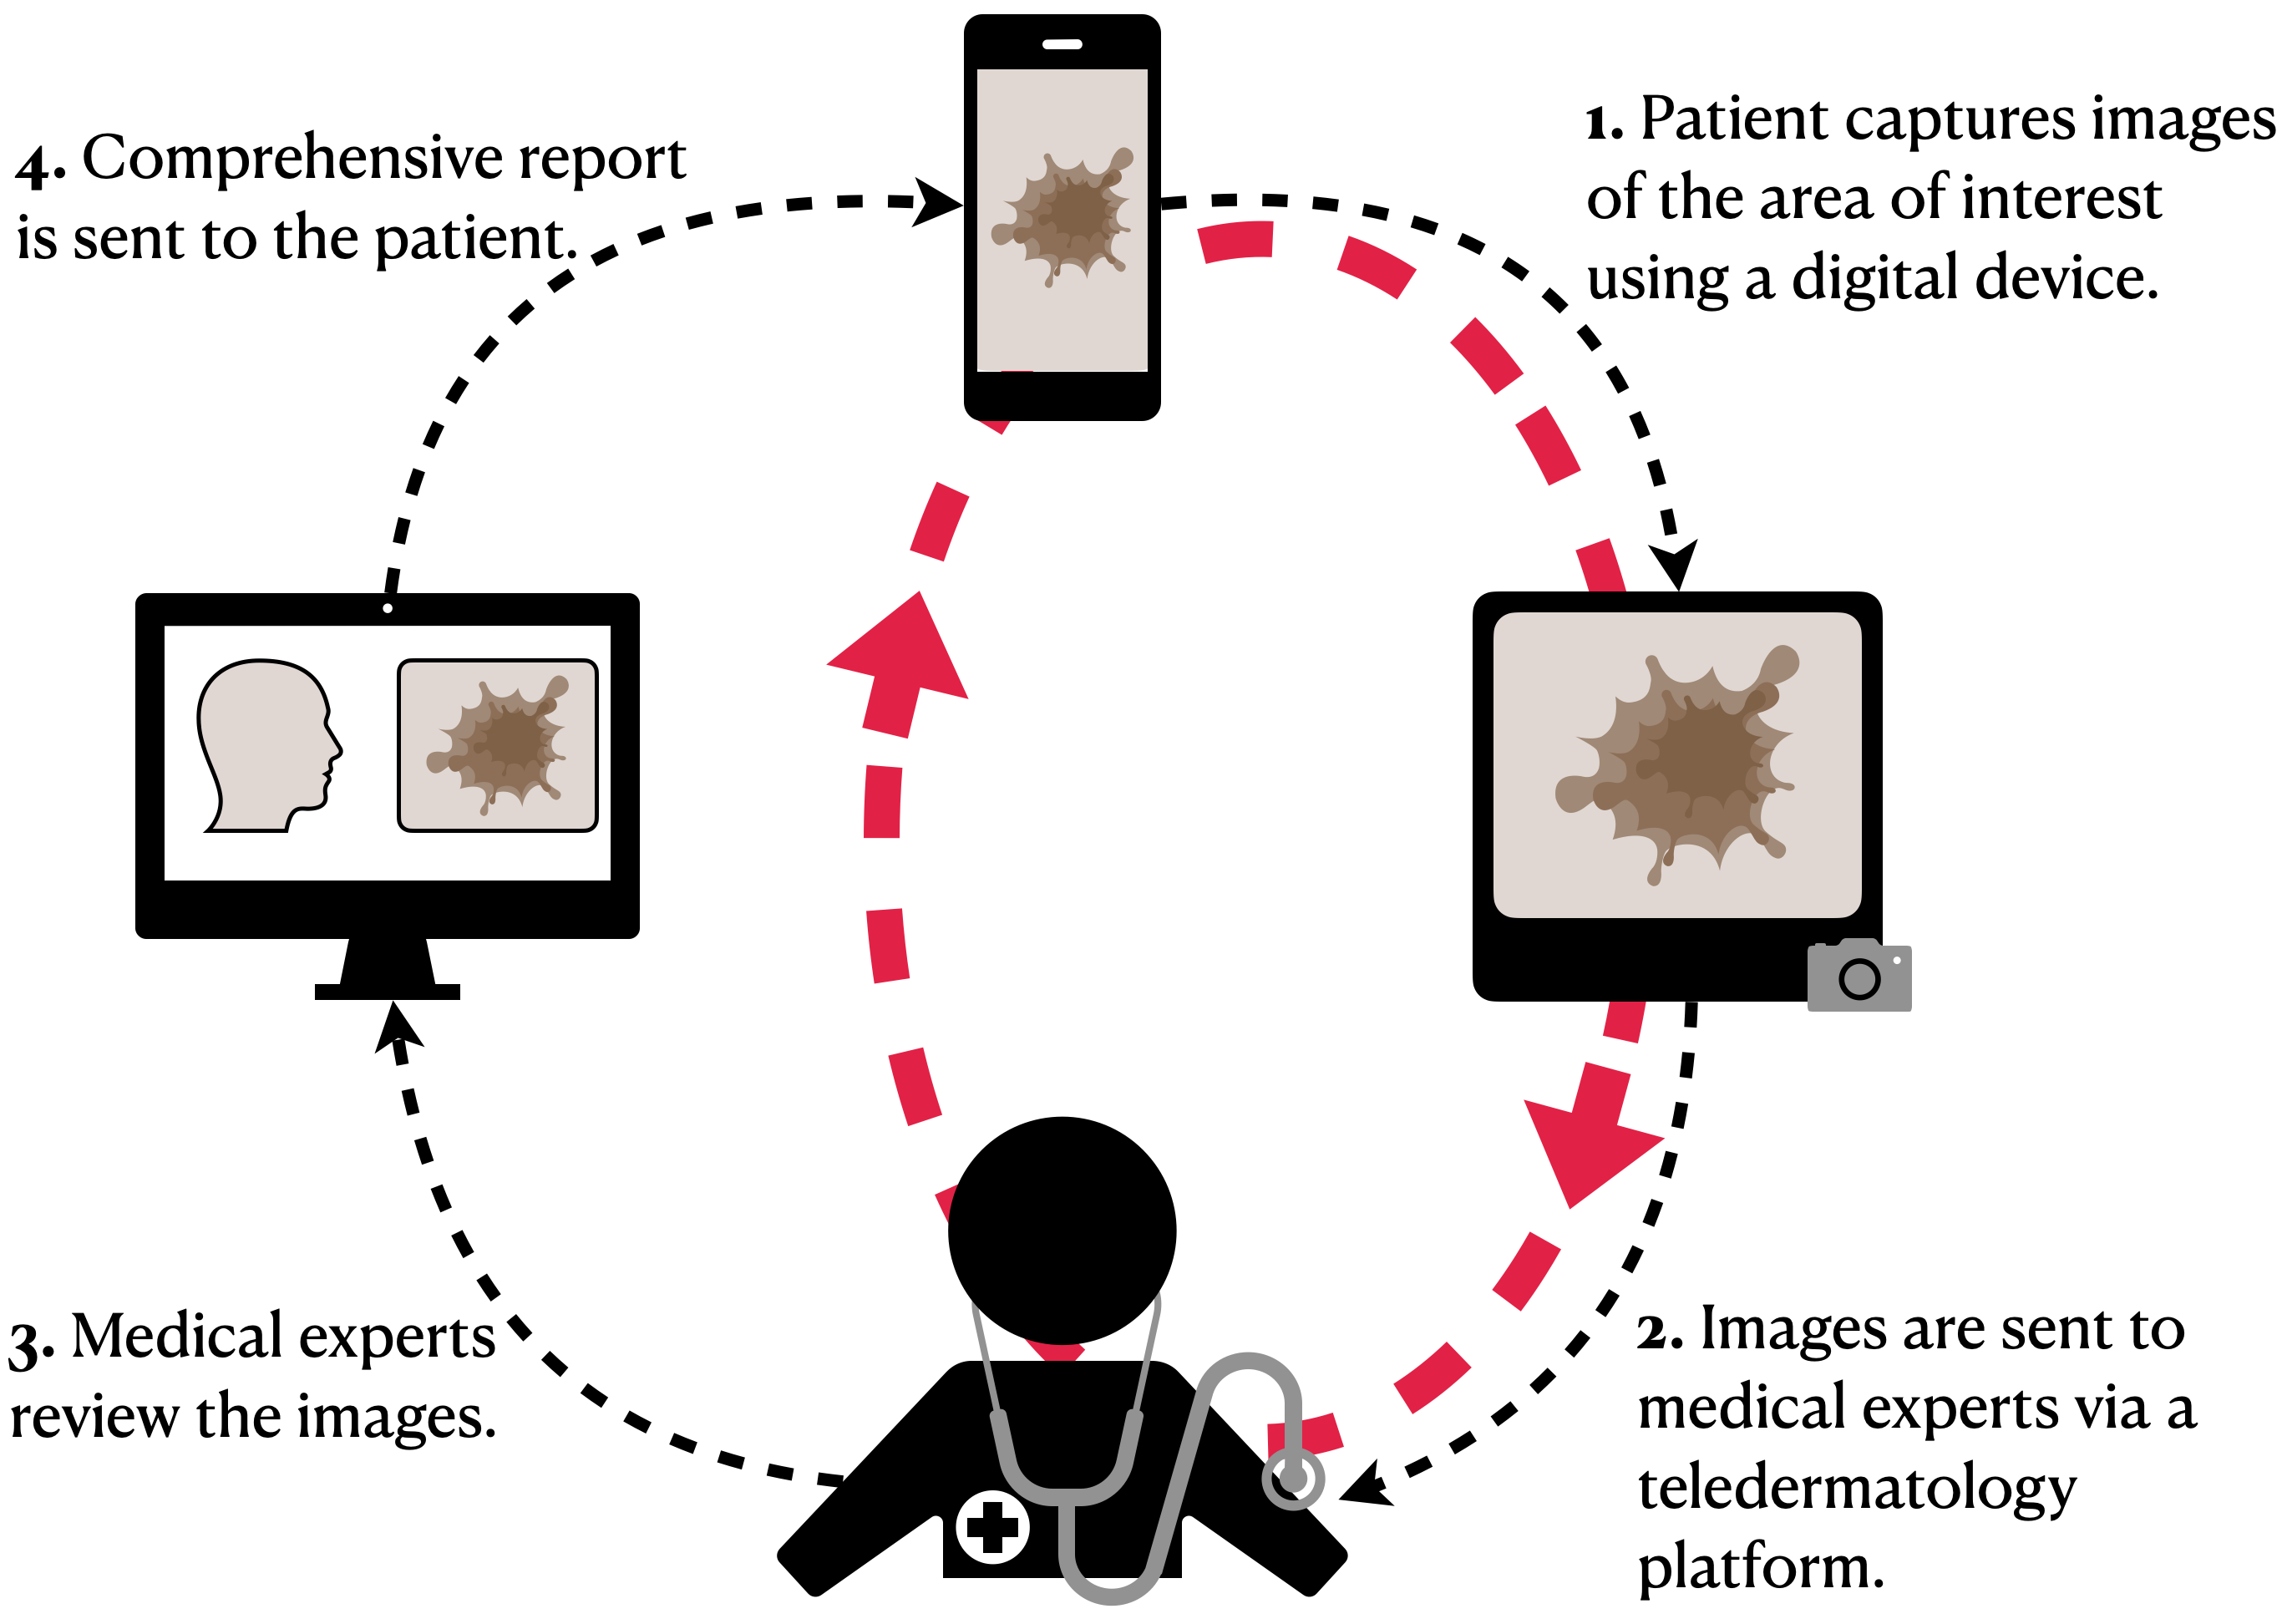
\includegraphics[keepaspectratio,width=15cm]{img/TD_workflow.png}
    \caption{This diagram illustrates the streamlined process of a teledermatology consultation, starting from the patient capturing images of their skin condition to the receipt of a detailed medical report. Each step highlights the essential role of image quality in ensuring accurate diagnosis and effective patient care. (Created by the Author)}
    \label{fig:TD_workflow}
\end{figure}
However, the success of teledermatology depends heavily on the quality of the images patients capture. Despite the convenience of modern technology, issues such as poor lighting, blurred images, and inadequate representation of skin conditions can greatly hinder a dermatologist's ability to make accurate diagnoses. These challenges with image quality reduce the effectiveness of teledermatology. \par
\vspace{\baselineskip}
Additionally, many images sent by patients do not meet the required standards. This common problem highlights the urgent need to improve the quality of images taken through mobile applications. Enhancing image clarity and accuracy is crucial for maintaining the reliability of diagnoses in teledermatology, and this thesis will explore the associated challenges and potential improvements in image quality within this field.\par 


\section{Objectives of the Thesis}
\label{sec:Objectives}
The primary aim of this thesis is to develop and evaluate automated methods for assessing image quality within the context of teledermatology. The objectives are multi-faceted, starting with a comprehensive literature review of image quality assessment (IQA) methods from the general imaging domain to assess their suitability for teledermatology applications. This thesis also aims to select appropriate quality metrics, apply these methods to relevant dermatological datasets, and establish a reproducible repository for future research. \par
\vspace{\baselineskip}
The specific objectives of this thesis are detailed as follows:
\begin{itemize}
    \item Literature Review: An extensive review of current image quality assessment methods will be conducted with a focus on their relevance and adaptability to teledermatology. This review will form the basis for developing specialized assessment techniques tailored for dermatological imagery.
    \item Identification of Image Quality Criteria: This will involve pinpointing specific image quality criteria that are essential for the accurate diagnosis of skin conditions via teledermatology. Setting these criteria is crucial for establishing standards and guidelines for image quality evaluation in a dermatological setting.
    \item Evaluation of Methods: This thesis will evaluate selected quality assessment methods using publicly available dermatological datasets. The evaluation will focus on the effectiveness and precision of these methods in objectively measuring image quality.
    \item Development of a Reproducible Repository: The creation of a well-documented and reproducible repository is planned. This repository will enable the reproduction of results and support the quality assessment of new patient images, serving as an invaluable resource for both researchers and practitioners in teledermatology.
\end{itemize}
Achieving these objectives is anticipated to significantly enhance the efficiency and accuracy of teledermatology services by establishing a standardized approach to image quality assessment. This standardization is expected to improve the workflow in teledermatology, providing effective tools and methodologies for evaluating the quality of patient images. Ultimately, the advancements from this research will contribute to better diagnostic precision and overall patient care in remote dermatological consultations. \par

\section{Organisation of this Thesis}
\label{sec:Structure}
This thesis is structured into six chapters to provide a clear and systematic exploration of image quality assessment in teledermatology. \autoref{ch:LiteratureReview} discusses the literature review, covering previous and related works on IQA and teledermatology. \autoref{ch:Methodology} details the methodologies used in the literature review, as well as those specific to IQA and teledermatology. In \autoref{ch:Implementation}, the experiments conducted are described, offering insights into the metrics used. \autoref{ch:ResultsAnalysis} presents the results of these investigations. Finally, \autoref{ch:DiscussionConclusion} concludes the thesis, summarizing the findings and suggesting directions for future research. \par